This section presents representative workflows that reflect common ocean and environmental science tasks.
The intent is not to prescribe a single ``best'' analysis path, but to illustrate how the \cmapagent\ (Fig.~\ref{fig:architecture}) turns natural-language intent into grounded, tool-executed operations with artifact-oriented outputs.
Across workflows, the agent (i) resolves datasets and variables using catalog-grounded context, (ii) executes validated operations through tools rather than free-form text, and (iii) returns persistent artifacts (data files, figures, and optional executable SDK code) to support reproducibility.

\subsection{Workflow 1: Concept-driven discovery and bounded data extraction}
Many sessions start with a scientific concept rather than a known table name.
For example, a user may ask for ``satellite chlorophyll concentration over the North Pacific Ocean'' or request candidate datasets for ``mixed-layer depth''.
The workflow proceeds in three stages:
\begin{enumerate}[leftmargin=*]
  \item \textbf{Concept-to-catalog grounding.} The agent retrieves relevant catalog context (dataset descriptions, variable lists, references) and proposes a small set of candidate datasets/variables.
  \item \textbf{Interactive disambiguation.} When multiple plausible candidates exist, the agent asks targeted follow-up questions (e.g., desired resolution, in-situ vs. gridded) to ensure the intended product is selected.
  \item \textbf{Bounded extraction as an artifact.} Once selected, the agent executes a spatiotemporal subset request and returns a downloadable artifact (e.g., CSV/Parquet) along with the bounds used and optional SDK code to reproduce the query.
\end{enumerate}
This pattern mirrors how scientists typically explore a portal: search, compare candidates, then extract a bounded subset for downstream analysis.
The key difference is that the interface is intent-first and grounded in the catalog, reducing the need for users to know internal identifiers up front.

\subsection{Workflow 2: Rapid visualization and climatological summaries}
Exploratory visualization is often the fastest way to validate whether a chosen dataset matches a hypothesis.
In \cmapagent, visualization requests are expressed at the level of scientific intent (map vs. time series; region vs. point; time range), and executed through deterministic plotting routines.
Two recurring patterns are:
\begin{enumerate}[leftmargin=*]
  \item \textbf{Quick-look plots from extracted subsets.} The agent produces maps or time series from a retrieved subset and returns the figure as an artifact, enabling immediate inspection and iteration.
  \item \textbf{Climatology and seasonal-cycle summaries.} For gridded products, users commonly request climatological means or seasonal cycles (e.g., ``mean monthly SST'' or ``seasonal chlorophyll'').
  The agent executes the corresponding aggregation, returns the derived dataset as an artifact, and generates a diagnostic plot that summarizes the seasonal structure.
\end{enumerate}
These outputs help users validate assumptions early (e.g., coverage, units, expected seasonality) before committing to larger analyses.
They also provide a bridge from conversational exploration to publication workflows by returning reusable artifacts and, optionally, executable code.

\subsection{Workflow 3: Dataset integration by colocalization}
Ocean science frequently requires integrating sparse in-situ observations with gridded satellite or model products.
CMAP provides a harmonized spatiotemporal index that supports this operation at scale \citep{Ashkezari2021SimonsCMAP}; \cmapagent\ makes the integration accessible through intent-level instructions.
In a typical colocalization workflow:
\begin{enumerate}[leftmargin=*]
  \item \textbf{Source selection.} The user specifies a source table (e.g., in-situ observations) and one or more target products (e.g., satellite SST), or provides a user-owned dataset as an uploaded artifact.
  \item \textbf{Tolerance specification.} The agent confirms spatial/temporal tolerances (and, where relevant, vertical matching assumptions) and validates that tolerances are within supported ranges.
  \item \textbf{Join execution and diagnostics.} The agent executes the join and returns an integrated table artifact, along with summary diagnostics (e.g., match counts, bounds used) and optional code for reuse.
\end{enumerate}
By returning the joined dataset as a file, the workflow supports downstream modeling, statistical analysis, and reproducible figure generation.
More broadly, it illustrates the core scientific promise of agentic interfaces: enabling multi-step, verifiable data operations without requiring users to manually orchestrate every intermediate command.

\subsection{Reporting provenance to support scientific trust}
Across workflows, the system can surface concise provenance: which dataset/variable candidates were considered, what bounds and tolerances were applied, and what artifacts were produced.
This emphasis on traceable, tool-executed trajectories aligns with broader findings in agent research that interleaving reasoning with actions can improve interpretability and reduce unsupported generation \citep{Yao2022ReAct}.
In \cmapagent, provenance also serves a practical purpose: it allows users to copy results into notebooks, share analyses with collaborators, and audit results when preparing figures for publication.


\subsection{Session vignettes with artifacts and provenance}
To avoid synthetic demonstrations, the paper will include short vignettes drawn from real \cmapagent\ sessions.
Each vignette reports (i) the user prompt, (ii) a compact provenance snippet summarizing tool calls and key parameters, and (iii) the resulting artifacts (e.g., tabular extracts and figures) suitable for direct reuse in notebooks.
The vignettes are intentionally brief and are meant to complement, not replace, the higher-level workflow descriptions above.

%\subsubsection*{Vignette 1: Concept-driven discovery and bounded extraction}
\begin{vignettebox}
\vignetteprompt{\textit{(User prompt)}}
\vignettefield{Condensed provenance}{\textit{(a compact tool-trace summary: tool names, key bounds/tolerances, and any dataset/variable resolutions.)}}
\vignettefield{Artifacts}{\textit{(List artifacts)}}
\end{vignettebox}


\subsubsection*{Vignette 1: Catalog discovery and visualization}
\begin{vignettebox}
\vignettefield{Prompt}{\textit{Make a Robinson-projected global map of total cloud cover in December 1945. Use an appropriate dataset available in CMAP and return the plot as an image.}}
\vignettefield{Condensed provenance}{Tools: Search Knowledge base, Plot map}
\vignettefield{Artifacts}{Python code to extract data, Download link to data, Generated visualization Fig.~\ref{fig:vin_viz}. }
\end{vignettebox}



\begin{figure}[t]
  \centering
  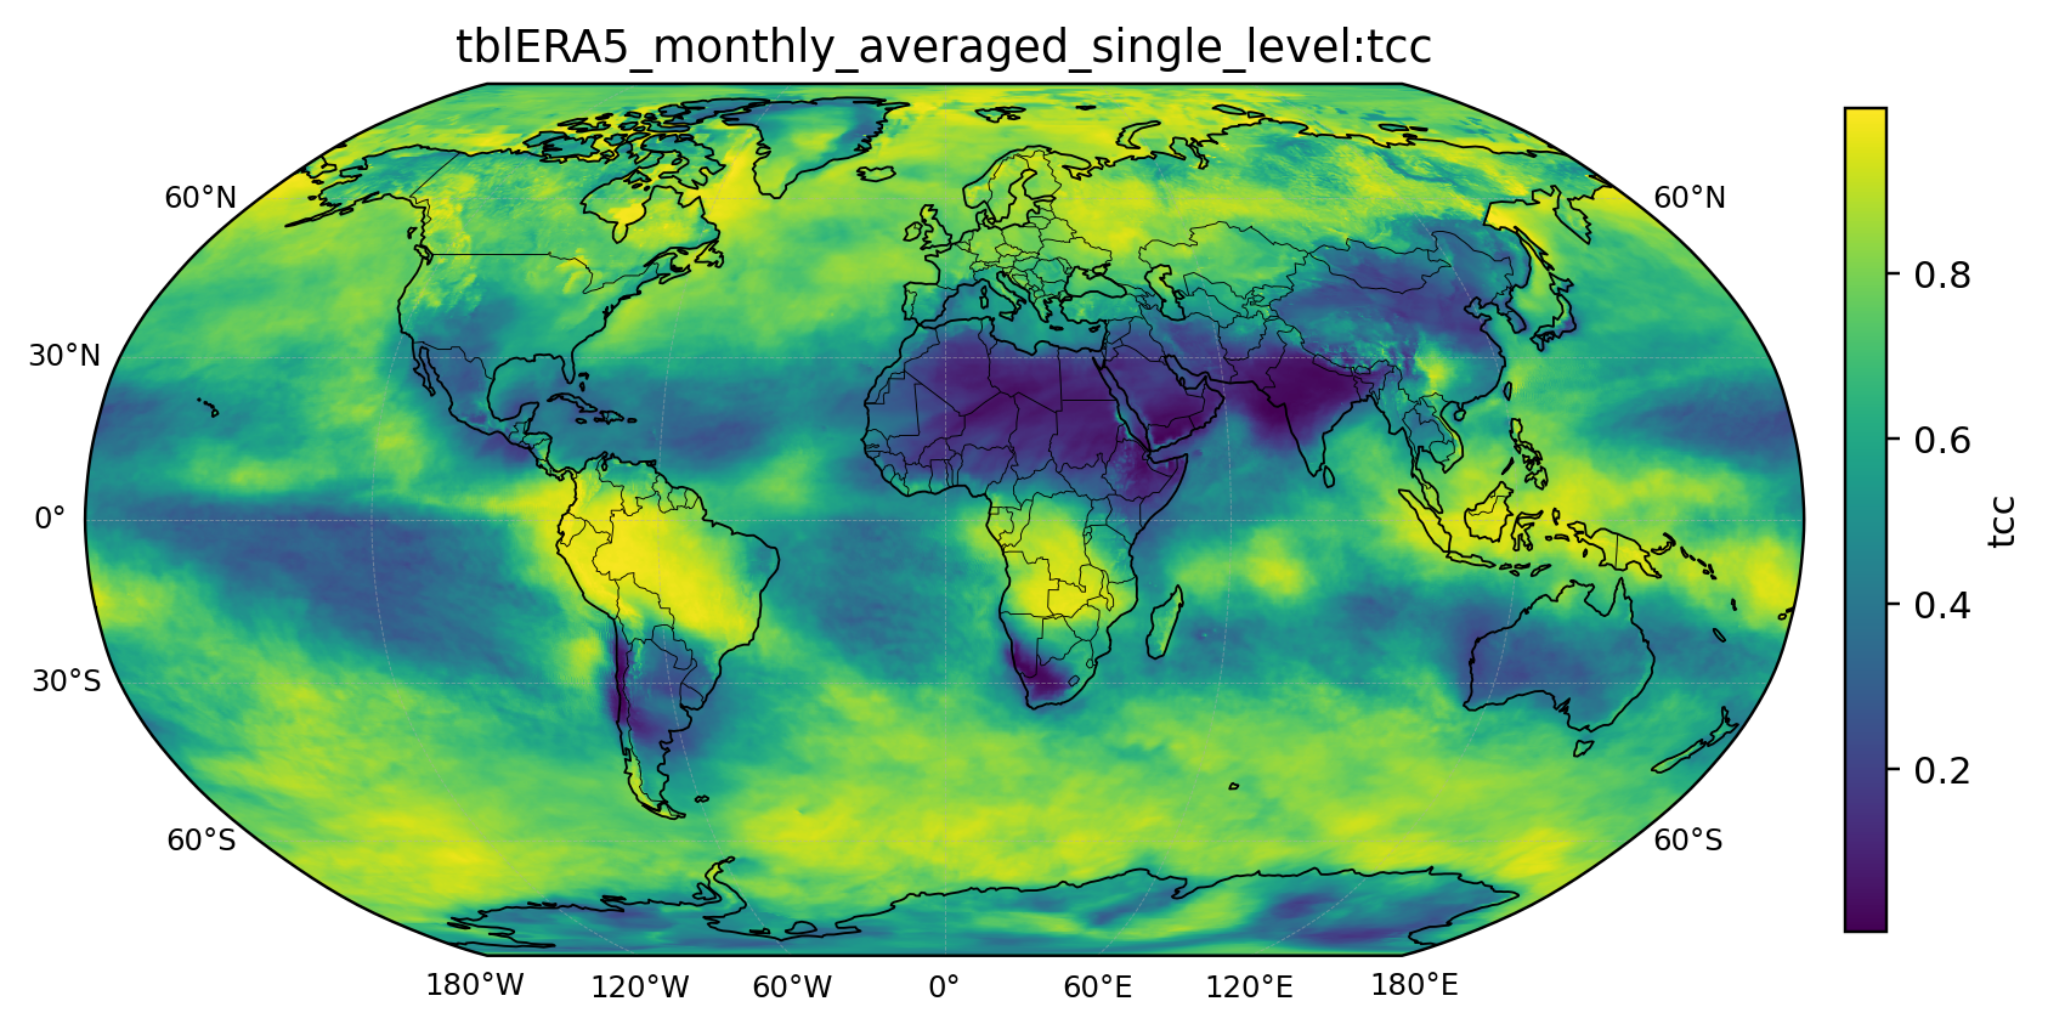
\includegraphics[width=\linewidth]{figures/tcc.png}
  \caption{Visualization workflow vignette. From a natural-language request, CMAP Agent generates a global map visualization of total cloud cover (tcc) for December 1945 from the ERA5 Monthly Averaged Single Levels dataset. Colors indicate cloud fraction, with coastlines and political boundaries overlaid for geographic context. The figure illustrates the agent’s ability to resolve a dataset/variable, retrieve the required subset, and produce a georeferenced map artifact that is returned as a downloadable figure file in a standard cartographic projection (Robinson)}
  \label{fig:vin_viz}
\end{figure}

\subsubsection*{Vignette 2: Dataset integration via co-localization}
\begin{vignettebox}
\vignettefield{Prompt}{\textit{Can you colocalize the 'Discrete Flow Cytometry of Underway Samples from TN427 Using a BD Influx Cell Sorter' dataset with: 
total precipitation (tp in tblERA5\_monthly\_averaged\_single\_level) from ERA5 dataset, 
and daily satellite SST (sst in tblSST\_AVHRR\_OI\_NRT), 
and Nitrate monthly climatology from the World Ocean Atlas 2013 v2 Climatology dataset (nitrate\_WOA\_clim in tblWOA\_Climatology)?}}
\vignettefield{Condensed provenance}{Tools: catalog search and colocalization}
\vignettefield{Artifacts}{python code for colocalization and the final integrated dataset is returned.}
\end{vignettebox}
